\subsection{Topology Protocol}
\label{proto_topo}

The \dcamp distributed topology is dynamically established as the Root node sends out its discovery message and receives
join messages from Base nodes. Once a Base node responds to the Root, the Base node is given its assignment.
Additionally, the Root node can shutdown the system using this same protocol but responding with a "stop" message
instead of an assignment.

\begin{figure}[H]
\vspace{+10pt}
\begin{verbatim}
topo-discovery = *discover join
discover       = R-MARCO
join           = B-POLO ( R-ASSIGN / R-STOP / R-WTF )
\end{verbatim}
\vspace{-5pt}
\caption[Topology Protocol]
        {Topology Protocol: \texttt{R-} represents the Root node sending a message and \texttt{B-}
         represents a Base node sending a message.}
\label{fig:proto_topo_spec}
\end{figure}

\begin{figure}[H]
    \centering
    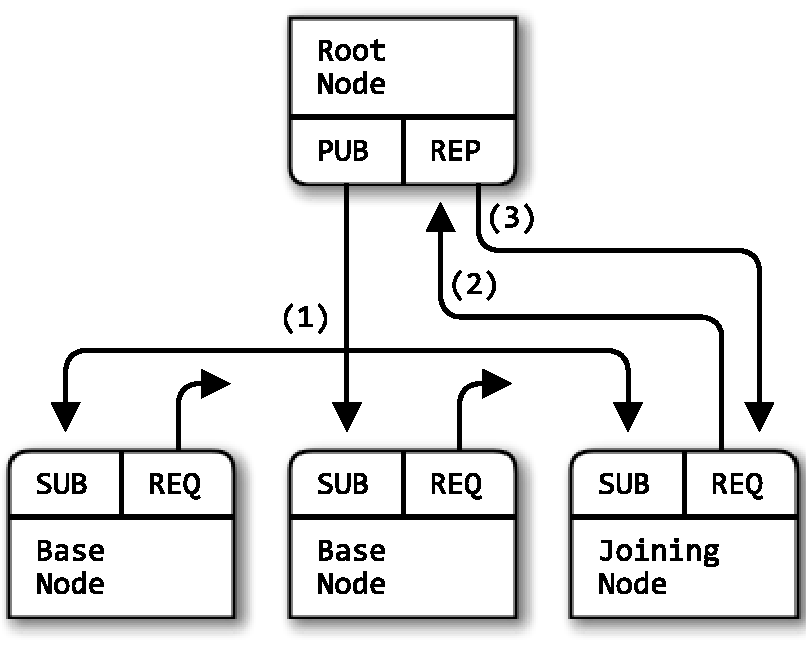
\includegraphics[scale=0.5]{topo.pdf}
    \label{fig:proto_topo_image}
    \caption{Topology Protocol Diagram}
\end{figure}

\subsubsection{Message Definitions}

\textbf{\texttt{TOPO}} is a generic topology message consisting of four frames. This message type is designed to be sent
across a PUB/SUB connection, from which subscribers filter incoming messages using the first frame. This design proves
useful for the \hyperref[proto_reco]{Recovery Protocols}.

The \texttt{MARCO} message is simply shorthand for \texttt{TOPO(key="/MARCO")}.

\begin{figure}[H]
\vspace{+10pt}
\begin{verbatim}
Frame 0: key, as 0MQ string
Frame 1: root address, as 0MQ string
Frame 2: root UUID, 16 bytes in network order
Frame 3: <empty> or content, as 0MQ string
\end{verbatim}
\vspace{-20pt}
\caption{\texttt{TOPO} Message Definition}
\label{fig:message_topo}
\end{figure}

\textbf{\texttt{CONTROL}} is a generic control message consisting of four frames and designed to be sent across a
REQ/REP connection. The \texttt{POLO}, \texttt{ASSIGN}, and \texttt{STOP} messages are shorthand for
\texttt{CONTROL(command="POLO")}, \texttt{CONTROL(command="ASSIGN")}, and \texttt{CONTROL(command="STOP")} respectively.

In the case of \texttt{ASSIGN}, the third frame contains the specific topology instructions (level-one collector, leaf
node, etc.) being sent to the Base node.

\begin{figure}[H]
\vspace{+10pt}
\begin{verbatim}
Frame 0: command, as 0MQ string
Frame 1: base address, as 0MQ string
Frame 2: base UUID, 16 bytes in network order
Frame 3: properties, JSON-encoded, as 0MQ string

command     = "polo" / "assignment"
properties  = *( parent / level / group )
parent      = "parent=" <node-address>
level       = "level=" ( "root" / "branch" / "leaf" )
group       = "group=" <group-identity>
\end{verbatim}
\vspace{-20pt}
\caption{\texttt{CONTROL} Message Definition}
\label{fig:message_control}
\end{figure}

\textbf{\texttt{WTF}} is \dcamp's error message type. It has three frames (though Frame 2 may be empty) with the first
designed to make error detection simple.

\begin{figure}[H]
\vspace{+10pt}
\begin{verbatim}
Frame 0: "WTF", as 0MQ string
Frame 1: error code, 4 bytes in network order
Frame 2: <empty> or error message, as 0MQ string
\end{verbatim}
\vspace{-20pt}
\caption{\texttt{WTF} Message Definition}
\label{fig:message_wtf}
\end{figure}
